\documentclass[main.tex]{subfiles}

\begin{document}

\section{Introduction}

\subsection{Background}

Cancer is the second most prevailing cause of death in the world, behind cardiovascular diseases. It was reported 14 million new cases of various cancers worldwide in 2019 \cite{cancer_number} and as life expectancy increase in the world, it is also expected for cancer rates to increase. There are several treatments for cancers, among them is \gls{rt}, a treatment developed in the early 1900s using x-rays to irradiate harmful tumours. \gls{rt} is an effective and non-invasive procedure, used to remove cancerous growth without surgical intervention. The main challenge of \gls{rt} is delivering a lethal dose to the tumour without harming healthy tissue in the patient. Children are especially vulnerable to the long term side effects of radiation therapy because of their bodies are not fully developed yet.

\begin{figure}[!ht]
    \centering
    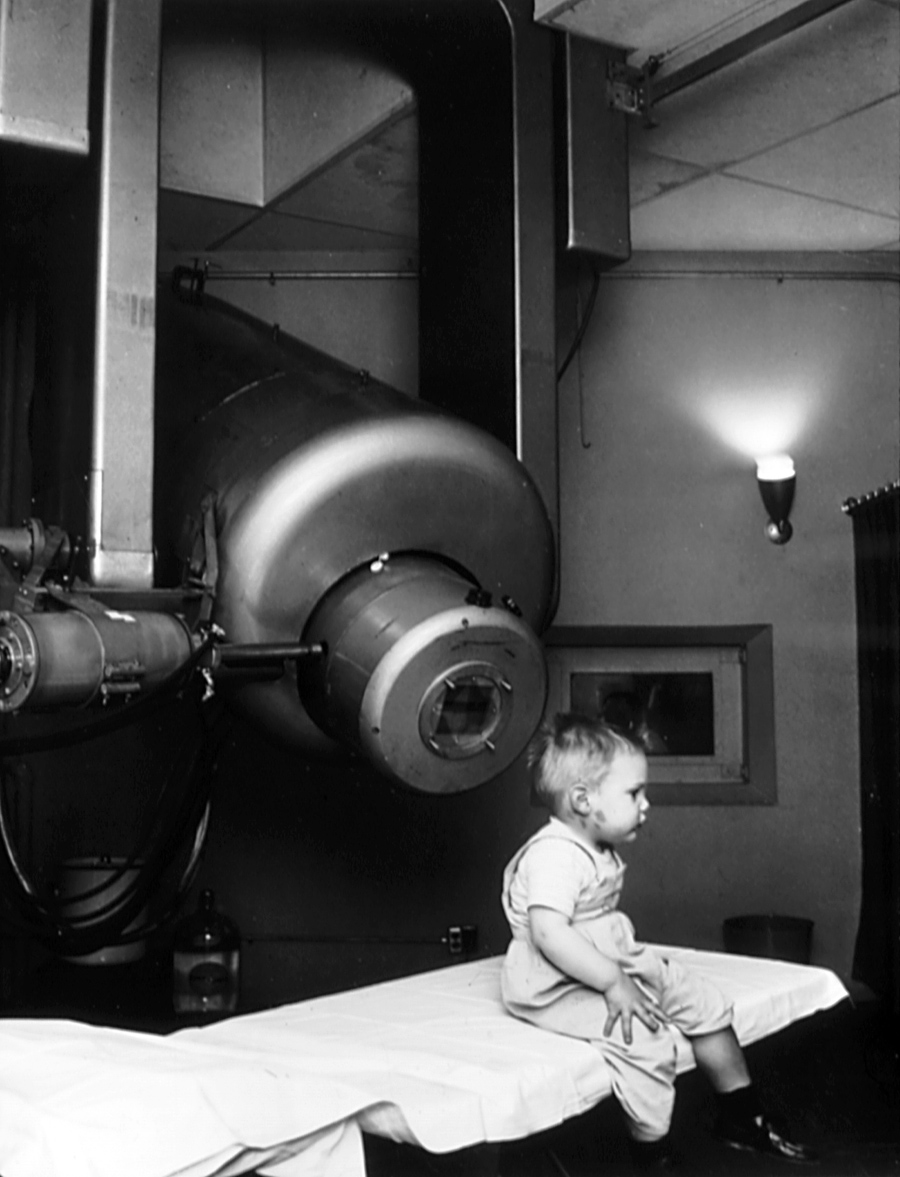
\includegraphics[scale = 0.4]{images/rt_intro.jpg}
    \caption{Image of the first pediatric patient being treated for retinoblastoma using radiotherapy.\cite{rt_intro}}
    \label{fig: rt_intro}
\end{figure}
\FloatBarrier


To calculate the dose distribution, a \gls{ct}-scan is performed before radiation therapy. A \gls{ct}-scan is done by sending X-rays through the patient, and detectors behind the patient measure the energy of the exiting photons. The density of the tissue is proportional to the absorption of the X-ray beams, meaning photons going through bone structures will lose most of their energy, while photons going through soft or no tissue will retain most of their energy. This property allows us to characterize the energy lost using the Hounsfield scale, a scale specifically designed for use in \gls{ct}-scans. With the Hounsfield scale, it is possible to create an image of the patient's insides, which can be used for diagnostics and can also be used to calculate the dose distribution. However, even with these techniques, the patient will still receive a significant radiation dose in adjacent tissue. Using \gls{rt} in high-risk areas, such as the brain or heart, can lead to severe damage to these organs.  \par

Particle therapy is a new treatment developed in the mid-1900s as an alternative to \gls{rt}. Particle therapy was sought as an alternative because particles allow for concentrating the dose distribution, which avoids damaging healthy tissue. Particles release very little energy while moving through a medium; it is not until the particle completely stops that it effectively releases all its energy. This phenomenon is known as "Bremsstrahlung", and it allows us to deliver high doses of energy to a concentrated area while having relatively little entry dose and effectively zero exit dose. The moment when the particle releases all its energy is known as the "Bragg-Peak", and we can calibrate this "peak", targeting only the tumour. Knowing the \gls{rsp} of the medium the particles are sent through is essential to control the Bragg-Peak. A traditional \gls{ct}-scanner can be used to calculate the \gls{rsp}; this is done by measuring the body's attenuation to radiation, measured in Hounsfield units, and converting the units into \gls{rsp}. However, the conversion from Hounsfield-units to \gls{rsp} is only an approximation, leading to higher uncertainty in the measurement. The stochastic nature of particles' energy loss also leads to higher uncertainties, making it even more crucial to have precise measurements when performing particle treatment. Directly measuring the \gls{rsp} with a particle \gls{ct}-scan can circumvent the uncertainty stemming from converting from Hounsfield units. This has led to further research and development of particle-based \gls{ct}-scan machines.


\subsection{Bergen PCT project}
Today the most common type of particle therapy is proton therapy; there are currently over 33 proton therapy centres in Europe. Norway plans to open two proton therapy centres by the end of 2024, one in Oslo and one in Bergen. The Bergen pCT-project is a collaboration with the University of Bergen and several other institutions to build a \gls{pct}-scanner to be used in particle therapy. The \gls{pct}-scanner is realized with a \gls{dtc} to measure the energy levels and trajectory of the protons exiting a patient exposed to a proton beam, to measure the \gls{rsp}.

\begin{figure}[!ht]
    \centering
    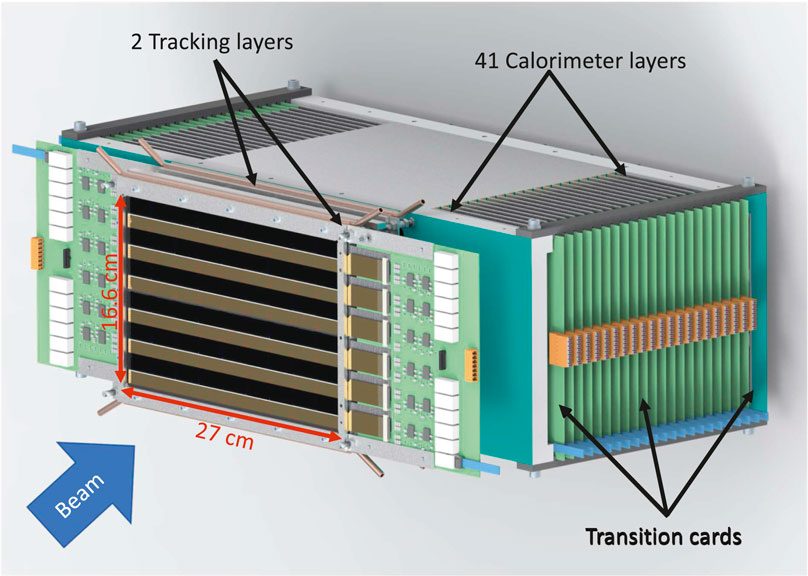
\includegraphics[scale = 0.5]{images/dtc.jpg}
    \caption{Image of the DTC to be used in the Bergen pCT project.}
    \label{fig: dtc_intro}
\end{figure}
\FloatBarrier

The \gls{dtc} is developed using \gls{alpide}-chips that was originally used for the \gls{its} in the \acrshort{alice} experiment at \acrshort{cern}. The \gls{dtc} is comprised of 43 layers, and each layer is assembled out of 12 strings with nine \gls{alpide}-chips each. The protons enter the front of the detector, and the chips measure their energy as they travel through each layer. 2 of the 43 layers are designated tracking layers, calculating the protons' trajectory when exiting the patient. It is necessary to track the angle of exiting protons due to effects such as coulomb-scattering, which affects the energy and trajectory of the protons. A \gls{dtc} is traditionally made with two tracking layers in the front and two layers in the rear of the \gls{dtc}, but the \gls{pct}-project only has the rear trackers. \textit{Single-sided} systems have advantages over \textit{double-sided} systems, such as reducing the cost and complexity of the system. A simplified block diagram of the \gls{pct} system is shown in \autoref{fig: dcs_renewed}.

\begin{figure}[!htpb]
    \centering
    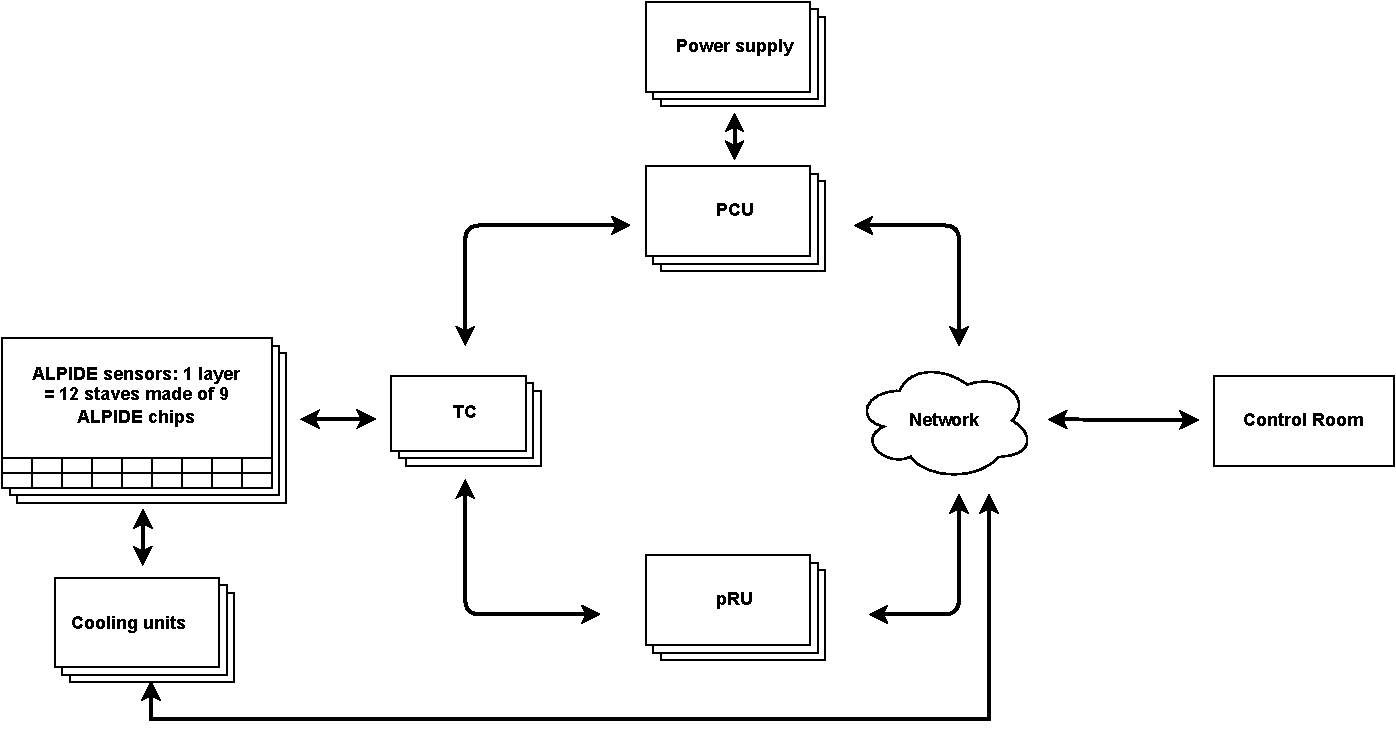
\includegraphics[scale = 0.65]{images/dcs_concept_renewed.pdf}
    \caption{Simplified block diagram of the pCT system.}
    \label{fig: dcs_renewed}
\end{figure}
\FloatBarrier

The figure shows the three systems encompassing the \gls{alpide} sensors, power delivery, readout, and cooling, all managed by the Control Room. The \gls{pcu} and \gls{pru} transfer power and perform readout of the strings, respectively, through the \gls{tc}s. Cooling is located next to the detector layers and is directly connected to the Control Room. All three systems are still in development; this thesis will focus on the power delivery system.

A separate \gls{mb} is responsible for delivering the power to the \gls{tc} and monitoring the temperature and current of the strings. Data transmission between the client and hardware is performed using IPbus, an established ethernet-based communication protocol developed for particle-physics experiments. The \gls{mb} must deliver enough current and monitor the temperature and current draw of the strings of \gls{alpide}-chips. The current plan is to have a power supply for each layer of the \gls{dtc} and an \gls{mb} for each layer to supply power and monitor the current draw. \par

The \gls{mb} uses a microcontroller to monitor the temperature and current draw of the layer; this allows us to quickly turn off strings if the temperature or current exceeds safe ranges. For this purpose, the microcontroller has several configurable registers for threshold values and readings of analogue current, digital current and temperature. The \gls{mb} requires a configuration system for safely powering the strings without damaging the equipment. A client-side monitoring system is also needed to give the user accurate information about the strings during a run. A monitoring system is essential for troubleshooting and debugging. The configuration and monitoring systems must also be able to quickly and reliably receive and transmit data between the user and the monitor boards, as slow configuration time could significantly impact the instrument's usability.

\subsection{Power Control and Monitoring}

The detector layer power system for the pCT requires both a configuration and a monitoring system. If the current consumption or temperature of the strings reaches a critical level, then they are turned off as fast as possible by the microcontroller. Additionally, there is a need for a control and monitoring system that interfaces with the \gls{mb} itself. The microcontroller must be configured through some process, and the system user needs a way to monitor the performance of the strings. It is common in the industry to use a standard for designing control systems called SCADA. Designing our control system using those standards is worthwhile to ensure the system is standardized and well-structured.

The configuration system must be able to configure the microcontroller with threshold values for current, voltage and temperature. Additionally, the system needs an algorithm for powering the strings one by one. Simultaneously turning on all strings will cause a large power spike, which can damage the equipment. The configuration system does not have a specific time constraint since the microcontroller takes care of time-critical events; however, the system should still not be too slow. The system should not be "laggy", meaning the computer should not lag when running the program, which is cumbersome for the user. Additionally, if the configuration process is slow, repeated troubleshooting becomes tedious, which should be avoided. Therefore the configuration should at at most, take 10 seconds to complete.

The monitoring system has similar requirements and no specific time constraint, but ideally, it should still be quick and not feel "laggy" to the user. The monitoring also has a polling frequency, determining how often it polls data from the microcontroller. The monitoring system should have a sampling frequency of a minimum 1Hz to get a good sampling of the power delivery parameters. However, a frequency of about 2-4Hz would be ideal for our system.

\subsection{Objective of this thesis}

This thesis aims to design and build the configuration and monitoring system for the \gls{pct} power delivery to the detector layers. Many aspects of the systems must be assessed and considered to ensure they are suitable for the \gls{pct}-project. Both systems must be able to communicate with the microcontroller on the monitoring board. As such, an \acrshort{fpga}-solution is used with IPbus to receive and transmit data between client software and the microcontrollers. \autoref{fig: pcs_basic} shows a block diagram of the power delivery system.

\begin{figure}[!htpb]
    \centering
    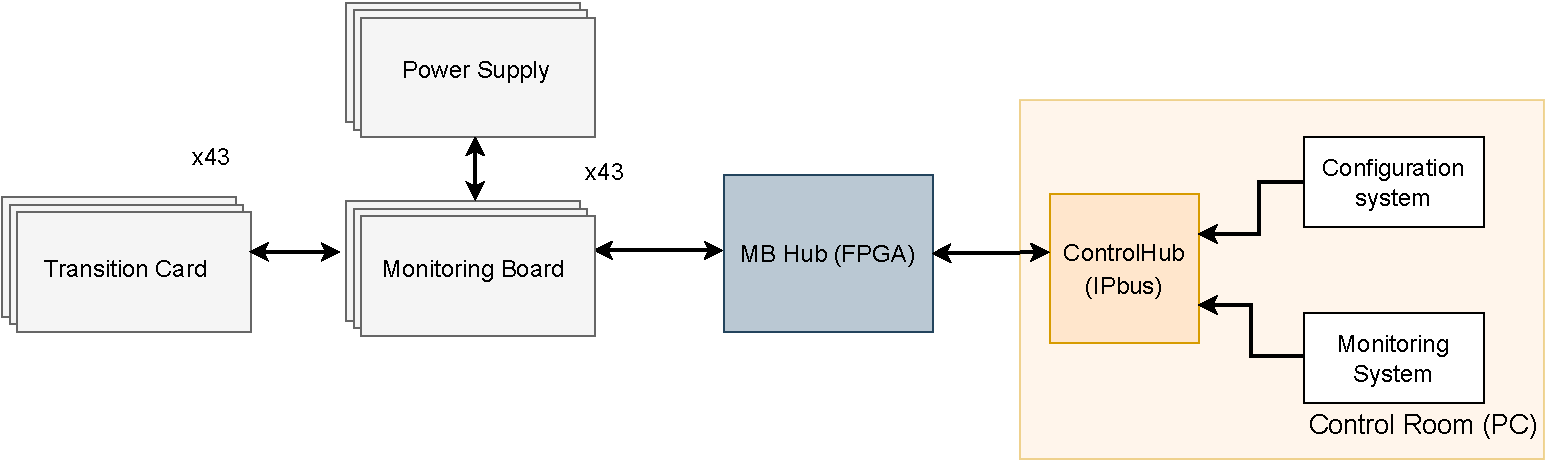
\includegraphics[scale = 0.65]{images/PCS basic overview.pdf}
    \caption{Block diagram of the power delivery system. The detector layers are directly connected to the TCs}
    \label{fig: pcs_basic}
\end{figure}
\FloatBarrier

The work will focus on creating the configuration and monitoring systems that will interface with the \gls{mb}s and the MB Hub. This involves creating an \gls{api} for the \gls{mb}s, a \gls{hmi} and databases for storing the data.

The work will use various software tools for communicating with IPbus and creating \gls{gui}s. The focus will be on creating a control system that is structured logically, modular, and generic. This will make the system easy to modify, expand upon, and reduce troubleshooting time, which is essential when working on an extensive control system. For example, the cooling and readout systems do not have a complete control system in place, but if the power control system is generic, then parts of that system can be reused for cooling and readout. The generic design would benefit the \gls{pct}-project because it would be simpler to manage three similar systems than three isolated, custom systems.


The requirements for this control system are as follows:

\begin{itemize}
    \item Configure all \gls{mb}s in the time span of 10 seconds. 
    \item Store configuration data in a database allowing for easy loading and saving configuration sets.
    \item A GUI that allows a user with little knowledge of the system to load configuration sets.
    \item A powering-on algorithm that turns on the strings one-by-one, leading to a slow ramp-up of power usage, to avoid creating a large power spike.
    \item Periodically read current draw and temperature from each layer and store the data in a time series database.
    \item Display the monitoring data from each layer in intuitive and easy-to-understand graphs.
    \item A low and high-level API to communicate with the IPbus module on the \gls{fpga} and the microcontroller on the \gls{mb}.
    \item Generic, modular \acrlong{oop} code that is easy to change and modify, so the system can be expanded upon and reused for similar projects in the future.
    \item The configuration process must not be "laggy" for the user and should not take more than a few seconds to complete.
    \item  The polling frequency of the monitoring process must be at least 1Hz, but ideally, it should be 2-4 Hz.
    \item The software design must follow software process standards and the SCADA control system standards.
    
The power system requires a low-level API that can perform basic communication with \gls{mb}, and this \gls{api} becomes the base interface for the other \gls{api}s for monitoring and configuration. Furthermore, following software process standards ensures that the system is structured logically, which helps the system be modular and generic. This means the system can be easily modified and expanded upon in future, which is a must for a control system with a long shelf time. Additionally, following the model for designing SCADA systems serves as a guideline for creating a structured and well-documented control system.
    
    
\end{itemize}

\newpage

\subsection{Structure of this thesis}

\textbf{Chapter 2 - Radiotherapy and Proton Therapy} \textit{This chapter goes through the theory of radiation and particle therapy and discusses the challenges with those treatments. The focus will be on how particle therapy can improve cancer treatment from traditional radiotherapy and what must be considered when using particle therapy.} 

\textbf{Chapter 3 - PCT project} \textit{This chapter introduces the \gls{pct}-project, the background of the project, and gives an overview of the different components and systems that comprises the \gls{pct}-project. It will discuss the calorimeter and the design of the detector layers. A description of the control system for power delivery and readout is given, and a general theory of control system development is discussed, focusing on SCADA systems.}

\textbf{Chapter 4 - PCS} \textit{This chapter will cover the power control system of the \gls{pct}-project. It will discuss the PCS's current design and describe its various parts. The chapter will discuss the design of the control software, the FPGA hub, and the monitor board of the PCS. The chapter will additionally cover the IPbus protocol, its characteristics and how it will be implemented in the control software.}

\textbf{Chapter 5 - Configuration System} \textit{This chapter will cover the design of the configuration system used in the power delivery system. It starts by going through the design of the configuration API and the layers of abstraction used in the lower-level API for the PCS. It will then cover the design requirements of the configuration system, such as the powering algorithm, the setup of the database, and the GUI that will interface with the entire system. It will also discuss the theoretical configuration timing of the system, along with the measured timing performed on the prototype setup.}

\textbf{Chapter 6 - Monitoring System} \textit{The chapter will go over the design of the monitoring system for the power delivery system. The monitoring API is covered, describing the hierarchy of API classes and their functions. The chapter will then cover the monitoring database and the various features and web interfaces used to display data in the monitoring system. It then describes the characteristics of the monitoring operation, such as polling speed and storage space. Finally, it discusses optimising data acquisition through filtering and batching data points.}

\textbf{Chapter 7 - Testing and Verification} \textit{The prototype setup of the PCS is introduced and various tests are described for testing the entire PCS chain. The results of those tests are discussed, and what they mean for the viability of the test setup. It will also go over simulation classes that were created to test API functionality with IPbus on software.}

\textbf{Chapter 8 - Discussion} \textit{This chapter discusses the work done in this thesis, what is incomplete or missing, and discusses how the work done for the power control system can be applied and reused for the other cooling and readout systems in the \gls{pct}-project.}

\textbf{Chapter 9 - Conclusion} \textit{This chapter sums up the work done in this thesis and details the future work that must be performed to make the system operational.}






\end{document}